\documentclass[11pt,a4paper]{article}

% --- Paquetes Esenciales ---
\usepackage[utf8]{inputenc}
\usepackage[spanish,es-tabla,es-nodecimaldot]{babel}
\usepackage[T1]{fontenc}
\usepackage{lmodern}
\usepackage{microtype}
\usepackage{graphicx}
\usepackage{xcolor}
\usepackage{tikz}
\usetikzlibrary{shapes,arrows,positioning,calc}
\usepackage[a4paper, top=2.5cm, bottom=2.5cm, left=2.3cm, right=2.3cm, headheight=22pt]{geometry}
\usepackage{fancyhdr}
\usepackage{tabularx}
\usepackage{booktabs}
\usepackage{tcolorbox}
\tcbuselibrary{skins,breakable}
\usepackage{enumitem}
\usepackage{caption}
\usepackage{subcaption}
\usepackage{titlesec}
\usepackage{hyperref}

% --- Paleta de Colores Inspirada en GameLluvia ---
\definecolor{NavyDark}{HTML}{0A1526}
\definecolor{NavyMedium}{HTML}{13283C}
\definecolor{NavyLight}{HTML}{233A52}
\definecolor{CyanGlow}{HTML}{218FCB}
\definecolor{CyanBright}{HTML}{67DCCE}
\definecolor{GoldDrop}{HTML}{D99E10}
\definecolor{RedAlert}{HTML}{B5394D}
\definecolor{PurpleItem}{HTML}{BD87E8}
\definecolor{GreenSafe}{HTML}{2E7D32}

% --- Configuración de Enlaces ---
\hypersetup{
    colorlinks=true,
    linkcolor=NavyMedium,
    urlcolor=CyanGlow,
    citecolor=NavyDark,
    pdftitle={Manual de Usuario - GameLluvia: Guardian de la Lluvia},
    pdfauthor={Rodrigo Escudero, Ariel Fuenzalida, Matias Santelices},
    pdfsubject={Manual de Usuario y Guia Oficial de Supervivencia},
    pdfkeywords={GameLluvia, LibGDX, Java, Manual de Usuario, Arcade}
}

% --- Estilo de Encabezados y Pies de Pagina ---
\pagestyle{fancy}
\fancyhf{}
\fancyhead[L]{\small\sffamily\color{NavyDark}\textbf{GameLluvia: Guardián de la Lluvia} \textcolor{NavyLight!60}{|} \textit{Manual de Usuario}}
\fancyhead[R]{\small\sffamily\color{NavyDark}\textbf{Versión 4.0}}
\fancyfoot[C]{\small\sffamily\color{NavyDark!70}--- Página \textbf{\thepage} ---}
\renewcommand{\headrulewidth}{0.8pt}
\renewcommand{\headrule}{\hbox to\headwidth{\color{CyanGlow}\leaders\hrule height \headrulewidth\hfill}}
\renewcommand{\footrulewidth}{0pt}

% --- Formato Elegante y Robusto de Secciones ---
\titleformat{\section}
  {\Large\sffamily\bfseries\color{NavyDark}}
  {\thesection.\ }
  {0.3em}
  {}
  [\vspace{-0.2em}\color{CyanGlow}\rule{\textwidth}{1.6pt}]

\titleformat{\subsection}
  {\large\sffamily\bfseries\color{NavyMedium}}
  {\thesubsection}{0.6em}
  {}[\vspace{-0.2em}\color{NavyLight!30}\rule{\textwidth}{0.6pt}]

\titleformat{\subsubsection}
  {\normalsize\sffamily\bfseries\color{NavyLight}}
  {\thesubsubsection}{0.6em}{}

% --- Cajas Temáticas Profesionales (tcolorbox) ---
\newtcolorbox{alerta}[2][]{
    enhanced,
    colback=RedAlert!6,
    colframe=RedAlert,
    arc=2mm,
    fonttitle=\bfseries\sffamily\color{white},
    title=#2,
    boxrule=1pt,
    left=10pt, right=10pt, top=6pt, bottom=6pt,
    #1
}

\newtcolorbox{consejo}[2][]{
    enhanced,
    colback=CyanBright!8,
    colframe=CyanGlow,
    arc=2mm,
    fonttitle=\bfseries\sffamily\color{white},
    title=#2,
    boxrule=1pt,
    left=10pt, right=10pt, top=6pt, bottom=6pt,
    #1
}

\newtcolorbox{tarjetaitem}[3][]{
    enhanced,
    colback=white,
    colframe=NavyLight!35,
    arc=2.5mm,
    boxrule=0.8pt,
    left=9pt, right=9pt, top=6pt, bottom=6pt,
    fonttitle=\bfseries\sffamily\color{NavyDark},
    title={\large #2 \hfill \normalsize\color{CyanGlow} #3},
    #1
}

\begin{document}

% ==============================================================================
% PORTADA
% ==============================================================================
\begin{titlepage}
\begin{tikzpicture}[remember picture, overlay]
    % Fondo base Azul Noche Profundo
    \fill[NavyDark] (current page.south west) rectangle (current page.north east);
    
    % Destello central
    \shade[inner color=CyanGlow!35, outer color=NavyDark!0] 
        ($(current page.center)+(0,3cm)$) circle (7.5cm);
        
    % Borde neón arcade
    \draw[CyanBright, line width=2pt] ($(current page.north west)+(1cm,-1cm)$) rectangle ($(current page.south east)+(-1cm,1cm)$);
    \draw[CyanGlow!40, line width=0.8pt] ($(current page.north west)+(1.15cm,-1.15cm)$) rectangle ($(current page.south east)+(-1.15cm,1.15cm)$);
\end{tikzpicture}

\vspace{0.6cm}
\begin{center}
    % Escudo o Cabecera
    
\includegraphics[height=2.2cm]{images/Escudo_PUCV.png}\\[0.4cm]
    {\sffamily\bfseries\color{CyanBright}\small PONTIFICIA UNIVERSIDAD CATÓLICA DE VALPARAÍSO}\\[0.1cm]
    {\sffamily\color{white!80}\small ESCUELA DE INGENIERÍA INFORMÁTICA \textcolor{CyanBright}{|} PROGRAMACIÓN AVANZADA}\\[1.4cm]

    % Título Principal Arcade
    \begin{tcolorbox}[
        enhanced,
        colback=NavyMedium!95,
        colframe=CyanBright,
        arc=4mm,
        width=0.92\textwidth,
        boxrule=1.8pt,
        halign=center
    ]
        \vspace{0.15cm}
        {\fontsize{32}{36}\selectfont\sffamily\bfseries\color{white} GAME / LLUVIA}\\[0.25cm]
        {\fontsize{19}{23}\selectfont\sffamily\bfseries\color{CyanBright} GUARDIÁN DE LA LLUVIA}\\[0.25cm]
        {\large\sffamily\color{GoldDrop}\textbf{MANUAL DE USUARIO Y GUÍA DE SUPERVIVENCIA}}
        \vspace{0.15cm}
    \end{tcolorbox}

    \vspace{0.7cm}
    % Captura Icónica del Juego en Portada
    \begin{tikzpicture}
        \node[inner sep=0pt, rounded corners=3mm, draw=CyanBright, line width=1.8pt] {
            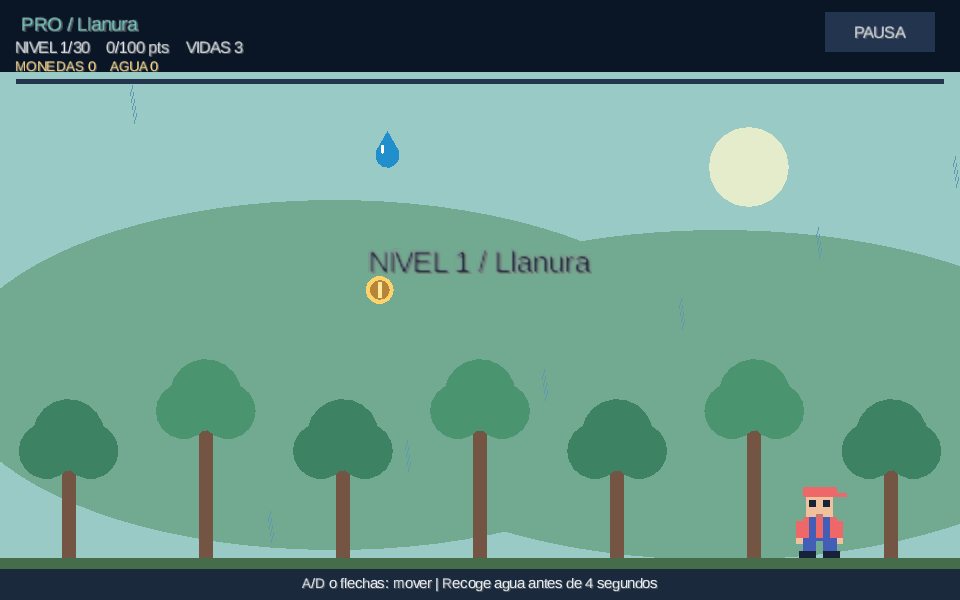
\includegraphics[width=0.72\textwidth]{images/02-partida.png}
        };
    \end{tikzpicture}

    \vfill

    % Datos del Equipo
    \begin{tcolorbox}[
        enhanced,
        colback=NavyDark!85,
        colframe=CyanGlow!70,
        arc=3mm,
        width=0.88\textwidth,
        boxrule=1pt
    ]
        \centering
        {\sffamily\bfseries\color{white}\small EQUIPO DE DESARROLLO}\\[0.15cm]
        {\sffamily\color{CyanBright}\textbf{Rodrigo Escudero}} \textcolor{white!60}{$\cdot$} 
        {\sffamily\color{CyanBright}\textbf{Ariel Fuenzalida}} \textcolor{white!60}{$\cdot$} 
        {\sffamily\color{CyanBright}\textbf{Matías Santelices S.}}\\[0.15cm]
        {\sffamily\color{white!70}\scriptsize Entorno: Java SE (JDK 17) + LibGDX 1.12.1 \textcolor{CyanBright}{|} Edición Cuarta Versión (Commit \texttt{af75f64})}
    \end{tcolorbox}
    \vspace{0.2cm}
\end{center}
\end{titlepage}

% ==============================================================================
% PAGINACION PARA EL CONTENIDO
% ==============================================================================
\setcounter{page}{1}

% ==============================================================================
% TABLA DE CONTENIDOS
% ==============================================================================
\vspace*{0.5cm}
\begin{center}
    {\Huge\sffamily\bfseries\color{NavyDark} Tabla de Contenidos}\\[0.2cm]
    {\color{CyanGlow}\rule{6cm}{2pt}}
\end{center}

\vspace{0.6cm}

\begin{tcolorbox}[
    enhanced,
    colback=white,
    colframe=NavyDark!30,
    arc=3.5mm,
    boxrule=1pt,
    left=16pt, right=16pt, top=14pt, bottom=14pt
]
{\large\sffamily\bfseries
\begin{enumerate}[label=\textbf{\arabic*.}, itemsep=0.9em]
    \item \hyperref[sec:intro]{Introducción y Contexto del Juego} \dotfill \pageref{sec:intro}
    \item \hyperref[sec:requisitos]{Requisitos del Sistema e Instalación} \dotfill \pageref{sec:requisitos}
    \item \hyperref[sec:objetivo]{Objetivo del Juego y Dinámica de Supervivencia} \dotfill \pageref{sec:objetivo}
    \item \hyperref[sec:controles]{Controles del Jugador y Modos de Juego} \dotfill \pageref{sec:controles}
    \item \hyperref[sec:interfaz]{Interfaz de Usuario (HUD y Menús)} \dotfill \pageref{sec:interfaz}
    \item \hyperref[sec:elementos]{Catálogo de Elementos y Precipitaciones (Guía de Campo)} \dotfill \pageref{sec:elementos}
    \item \hyperref[sec:campana]{Progresión de Campaña: Biomas y Batalla Final con el OVNI} \dotfill \pageref{sec:campana}
    \item \hyperref[sec:tienda]{Tienda de Aspectos, Personalización y Desbloqueos} \dotfill \pageref{sec:tienda}
    \item \hyperref[sec:faq]{Preguntas Frecuentes y Solución de Problemas (FAQ)} \dotfill \pageref{sec:faq}
\end{enumerate}
}
\end{tcolorbox}

\vspace{0.6cm}
\begin{center}
    \begin{tikzpicture}
        \node[inner sep=0pt, rounded corners=3mm, draw=NavyLight!40, line width=1pt] {
            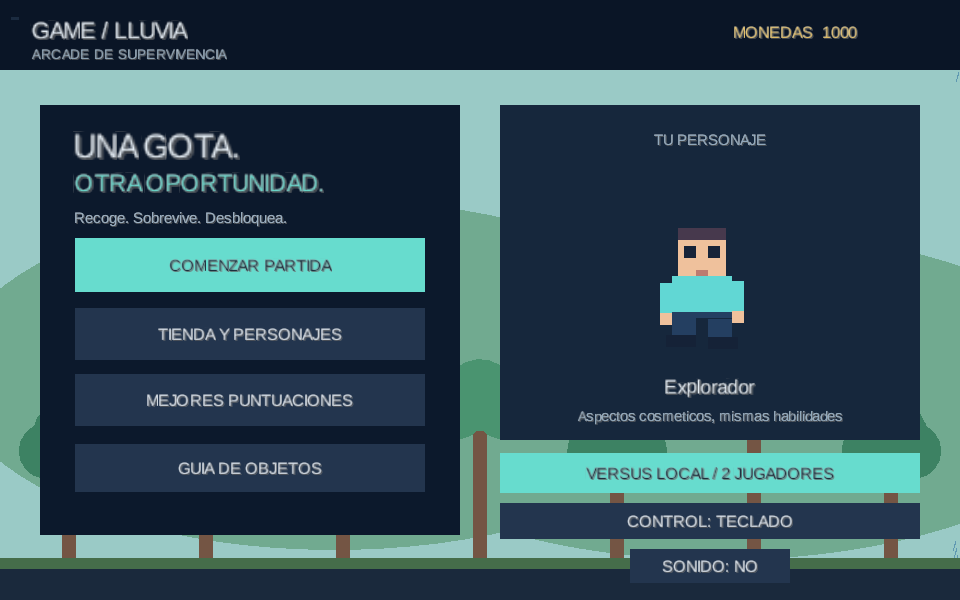
\includegraphics[width=0.85\textwidth]{images/01-menu.png}
        };
    \end{tikzpicture}\\[0.2cm]
    {\small\sffamily\color{NavyDark!70}\textit{Figura: Pantalla principal de acceso a todos los módulos y modos del videojuego.}}
\end{center}

\newpage

% ==============================================================================
% SECCION 1: INTRODUCCION
% ==============================================================================
\section{Introducción y Contexto del Juego}
\label{sec:intro}

En un planeta azotado por una catástrofe ambiental y una sequía implacable, la atmósfera se ha desestabilizado por completo. Las lluvias torrenciales ya no son un fenómeno cotidiano, sino un acontecimiento extraordinario cargado de esperanza y peligro a partes iguales.

Tú encarnas al \textbf{Guardián de la Lluvia}, un intrépido recolector equipado con un recipiente de flujo dinámico cuya misión prioritaria es cosechar cada gota de agua cristalina y nutrientes benéficos que descienden de las nubes antes de que se pierdan en la tierra estéril o se contaminen.

\begin{center}
    \begin{minipage}{0.48\textwidth}
        \begin{tcolorbox}[colback=white, colframe=CyanGlow, arc=2mm, boxrule=0.8pt, title=\textbf{La Amenaza del Espacio Exterior}]
            \small
            La situación climática empeora drásticamente cuando los radares detectan una enorme nave nodriza extraterrestre: el \textbf{Jefe OVNI}. Esta entidad alienígena desciende sobre la Tierra con el único fin de succionar las últimas reservas hídricas del planeta mediante rayos tractores atmosféricos.
        \end{tcolorbox}
    \end{minipage}
    \hfill
    \begin{minipage}{0.48\textwidth}
        \begin{tcolorbox}[colback=white, colframe=GoldDrop!90!black, arc=2mm, boxrule=0.8pt, title=\textbf{El Deber del Guardián}]
            \small
            Para detener la extinción, el Guardián debe atravesar \textbf{30 niveles} divididos en 3 biomas extremos, sobrevivir a precipitaciones tóxicas, acumular suficiente agua a presión y finalmente ascender a la estratosfera para expulsar al invasor espacial.
        \end{tcolorbox}
    \end{minipage}
\end{center}

\vspace{0.4cm}

\begin{figure}[h!]
    \centering
    \begin{subfigure}[b]{0.48\textwidth}
        \centering
        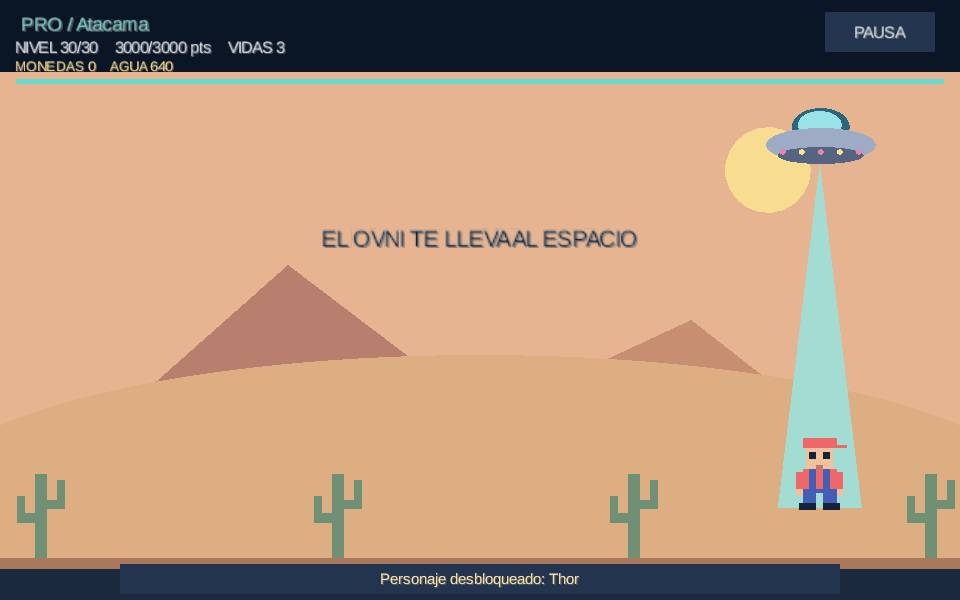
\includegraphics[width=\textwidth]{images/14-ascenso.png}
        \caption{Transición y ascenso a la atmósfera orbital}
    \end{subfigure}
    \hfill
    \begin{subfigure}[b]{0.48\textwidth}
        \centering
        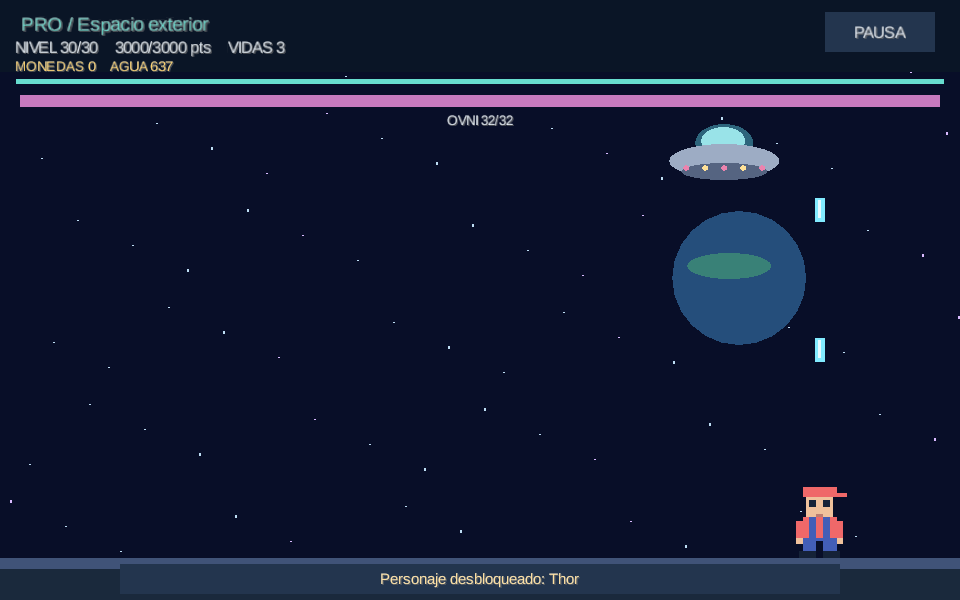
\includegraphics[width=\textwidth]{images/15-jefe.png}
        \caption{Confrontación decisiva contra la nave invasora}
    \end{subfigure}
    \caption{El clímax de la aventura: desde la recolección terrestre hasta el combate espacial.}
\end{figure}

\newpage

% ==============================================================================
% SECCION 2: REQUISITOS DEL SISTEMA E INSTALACION
% ==============================================================================
\section{Requisitos del Sistema e Instalación}
\label{sec:requisitos}

\textbf{GameLluvia} ha sido desarrollado sobre el motor multiplataforma \textbf{LibGDX} en lenguaje Java, con una versión Desktop probada en Windows y JDK 17. El juego limita los cuadros a 60 por segundo; el rendimiento depende del equipo. Android y otros sistemas requieren validación específica.

\subsection*{Especificaciones Técnicas del Sistema}

\begin{table}[h!]
\centering
\begin{tcolorbox}[enhanced, colback=white, colframe=NavyMedium, arc=3mm, boxrule=1pt, width=\textwidth, left=4pt, right=4pt, top=4pt, bottom=4pt]
\begin{tabularx}{\textwidth}{lXX}
\toprule
\textbf{Componente} & \textbf{Requisitos Mínimos} & \textbf{Requisitos Recomendados} \\
\midrule
\textbf{Sistema Operativo} & Windows probado & Linux/macOS requieren validación específica \\
\textbf{Procesador y RAM} & No se midió un mínimo & Probar en el equipo de evaluación \\
\textbf{Almacenamiento} & Fuentes, assets y dependencias & Gradle descarga bibliotecas la primera vez \\
\textbf{Entorno Java} & JDK 17 usado en pruebas & Gradle Wrapper 8.10.1 incluido \\
\textbf{Gráficos} & Controladores compatibles con LWJGL3 & Comprobar que abre sin errores \\
\textbf{Resolución Lógica} & $960 \times 600$ & Ventana escalable con bandas \\
\bottomrule
\end{tabularx}
\end{tcolorbox}
\caption{Ficha técnica de requerimientos para la versión de escritorio.}
\end{table}

\subsection*{JAR de la entrega final}
La preparación final agrega \texttt{.\textbackslash gradlew.bat :lwjgl3:dist}. El archivo \texttt{lwjgl3/build/libs/GameLluvia.jar} incluye librerías y assets. Se ejecuta con \texttt{java -jar GameLluvia.jar}, con Java instalado.
\subsection*{Guía de Puesta en Marcha Rápida}

El proyecto incluye scripts que requieren JDK 17 y conexión para descargar dependencias en su primera ejecución. La distribución también requiere Java instalado:

\begin{enumerate}[label=\textbf{\arabic*.}, itemsep=0.8em]
    \item \textbf{Ejecución Inmediata en Windows (Recomendada):}\\
    Navegue a la carpeta raíz del proyecto y haga doble clic sobre el archivo \textbf{\texttt{JUGAR.bat}}. Este script compila y ejecuta de manera autónoma el módulo de escritorio.
    
    \item \textbf{Ejecución desde Consola de Comandos o Terminal:}\\
    Si prefiere ejecutar mediante terminal o utiliza Linux/macOS, abra una consola en la raíz del proyecto y escriba:
    \begin{tcolorbox}[colback=NavyDark, colframe=CyanGlow, arc=1.5mm, boxrule=0.8pt, left=8pt, right=8pt, top=4pt, bottom=4pt]
        \color{CyanBright}\texttt{.\textbackslash gradlew.bat :lwjgl3:run} \quad \textcolor{white!70}{(En Windows PowerShell o CMD)}\\
        \color{CyanBright}\texttt{./gradlew :lwjgl3:run} \quad \textcolor{white!70}{(En Linux o macOS Bash/Zsh)}
    \end{tcolorbox}

    \item \textbf{Generación de Distribución de Escritorio:}\\
    Para empaquetar el juego y distribuirlo sin requerir el código fuente, ejecute:
    \begin{tcolorbox}[colback=NavyDark, colframe=CyanGlow, arc=1.5mm, boxrule=0.8pt, left=8pt, right=8pt, top=4pt, bottom=4pt]
        \color{CyanBright}\texttt{.\textbackslash gradlew.bat :lwjgl3:installDist}
    \end{tcolorbox}
    Los scripts y bibliotecas se encontrarán en \texttt{lwjgl3/build/install/lwjgl3/}.
\end{enumerate}

\begin{consejo}{Ajuste Dinámico de Pantalla y Proporción (FitViewport)}
    El juego opera internamente bajo una resolución virtual fija de \textbf{$960 \times 600$ píxeles}. Gracias al sistema \texttt{FitViewport}, usted puede maximizar la ventana o redimensionarla libremente en cualquier monitor panorámico ($16:9$, $16:10$, $21:9$); el motor mantendrá la proporción original perfecta proyectando bandas negras protectoras sin deformar la imagen.
\end{consejo}

\newpage

% ==============================================================================
% SECCION 3: OBJETIVO DEL JUEGO Y DINAMICA DE SUPERVIVENCIA
% ==============================================================================
\section{Objetivo del Juego y Dinámica de Supervivencia}
\label{sec:objetivo}

En \textbf{GameLluvia}, controlas a tu personaje desplazándolo horizontalmente por la parte baja del escenario. El objetivo primordial es recolectar la mayor cantidad de gotas benéficas, mantener saciada la sed del personaje, esquivar sustancias letales y acumular puntuación para ascender a través de los \textbf{30 niveles de la campaña principal}.

\begin{center}
    \begin{tikzpicture}
        \node[inner sep=0pt, rounded corners=3mm, draw=CyanGlow, line width=1.5pt] {
            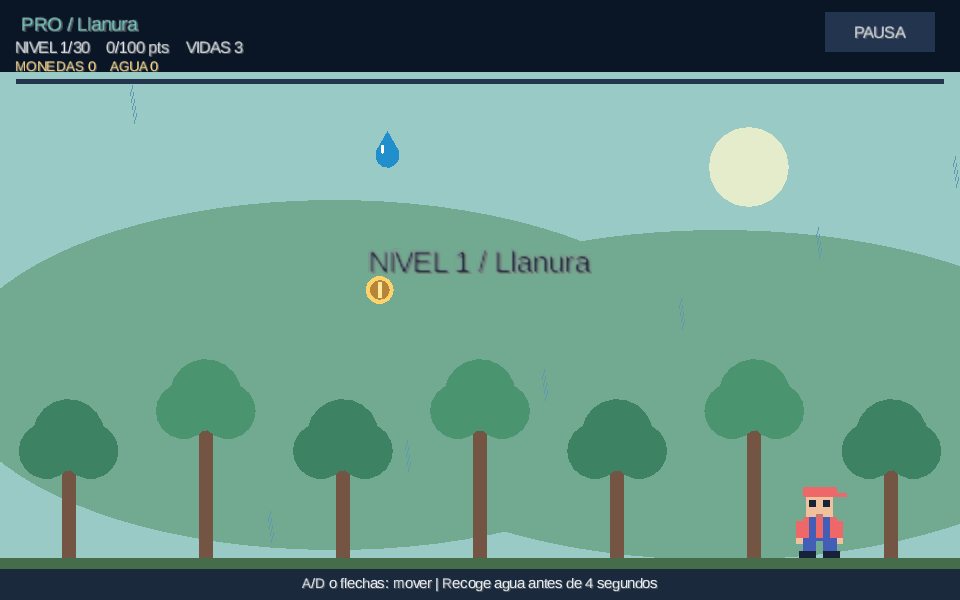
\includegraphics[width=0.82\textwidth]{images/02-partida.png}
        };
    \end{tikzpicture}\\[0.2cm]
    {\small\sffamily\color{NavyDark!70}\textit{Figura: Partida activa en el bioma de Llanura, capturando gotas y vigilando el estado de sed.}}
\end{center}

\subsection*{Las Reglas Fundamentales de Juego}

\begin{itemize}[itemsep=0.6em]
    \item \textbf{Captura y Avance de Niveles:} Cada gota de agua pura que cae y es atrapada suma \textbf{10 puntos} y recarga tu tanque de agua. Cada \textbf{100 puntos} acumulados, el jugador sube inmediatamente de nivel, acelerando el ritmo de la tormenta.
    \item \textbf{Peligros y Contaminantes:} Los elementos dañinos no solo restan puntos (pudiendo hacer descender tu progreso numérico), sino que los tóxicos como el ácido, el fuego o los cactus consumen directamente una de tus \textbf{vidas}.
    \item \textbf{Condición de Derrota:} Si tu contador de vidas llega a cero ($0$), la partida finaliza de inmediato (Game Over) y tus puntos se registrarán en la tabla histórica de récords.
    \item \textbf{Condición de Victoria:} Superar los 3.000 puntos en el nivel 30 y destruir a la nave nodriza en el combate espacial de la fase final.
\end{itemize}

\subsection*{La Mecánica Crítica de la Sed (Deshidratación)}

A diferencia de los arcades tradicionales, el recolector es un ser vivo que consume energía rápidamente bajo la atmósfera hostil. Si descuidas la ingesta de agua, el personaje sufrirá fatiga por deshidratación:

\begin{alerta}{¡Cuidado con la Sed Prolongada!}
    \textbf{¿Qué ocurre a los 4 segundos sin agua?} \\
    Si transcurren más de \textbf{4 segundos continuos} sin atrapar una sola gota de agua limpia, el personaje empieza a experimentar fatiga severa. Por cada segundo adicional, su velocidad de traslación se reduce un 15\%, acumulando hasta una \textbf{penalización máxima del 60\% de lentitud}. \\
    Quedar ralentizado en medio de una tormenta de ácido es una sentencia de muerte. \textbf{Para restaurar tu velocidad máxima al 100\%, basta con atrapar cualquier gota de agua fresca}.
\end{alerta}

\subsection*{Niveles de Dificultad}

Antes de comenzar cada aventura, el jugador puede elegir entre tres modalidades adaptadas a su nivel de habilidad:

\begin{table}[h!]
\centering
\begin{tcolorbox}[enhanced, colback=white, colframe=NavyDark, arc=3mm, boxrule=1pt, width=\textwidth, left=4pt, right=4pt, top=4pt, bottom=4pt]
\begin{tabularx}{\textwidth}{lcXX}
\toprule
\textbf{Dificultad} & \textbf{Vidas Iniciales} & \textbf{Comportamiento de la Tormenta} & \textbf{Perfil del Jugador} \\
\midrule
\textbf{NOOB} & \textbf{5 Vidas} & Ritmo suave, menor frecuencia de proyectiles dañinos y tiempo de reacción amplio. & Ideal para principiantes y para aprender los efectos de cada gota. \\
\textbf{PRO} & \textbf{3 Vidas} & Lluvia rápida, balance equilibrado de mejoras y amenazas con caída acelerada. & Experiencia intermedia; dispone de un ranking local por dificultad. \\
\textbf{HACKER} & \textbf{1 Sola Vida} & Caída frenética y reflejos extremos. \textbf{Un solo impacto letal causa derrota inmediata}. & Diseñado exclusivamente para veteranos en busca del récord perfecto. \\
\bottomrule
\end{tabularx}
\end{tcolorbox}
\caption{Comparativa de dificultades disponibles en el menú de selección.}
\end{table}

\newpage

% ==============================================================================
% SECCION 4: CONTROLES DEL JUGADOR Y MODOS DE JUEGO
% ==============================================================================
\section{Controles del Jugador y Modos de Juego}
\label{sec:controles}

El sistema implementa el patrón de arquitectura \textbf{Strategy}, lo que permite seleccionar un esquema de movimiento al iniciar la partida.

\subsection*{Esquema de Controles en Modo Solitario}

\begin{table}[h!]
\centering
\begin{tcolorbox}[enhanced, colback=white, colframe=CyanGlow, arc=3mm, boxrule=1pt, width=\textwidth, left=6pt, right=6pt, top=6pt, bottom=6pt]
\begin{tabularx}{\textwidth}{p{3.8cm}p{4.2cm}X}
\toprule
\textbf{Acción} & \textbf{Teclas de Entrada} & \textbf{Descripción Operativa} \\
\midrule
\textbf{Moverse a la Izquierda} & \texttt{FLECHA IZQUIERDA} ó \texttt{A} & Desplaza al recolector hacia el borde izquierdo. \\
\textbf{Moverse a la Derecha} & \texttt{FLECHA DERECHA} ó \texttt{D} & Desplaza al recolector hacia el borde derecho. \\
\textbf{Disparar Cañón de Agua} & \texttt{BARRA ESPACIADORA} / \texttt{CLIC} & Lanza chorros de agua a presión contra el OVNI (requiere agua acumulada). \\
\textbf{Pausar / Reanudar} & \texttt{P} ó \texttt{ESCAPE} & Congela la simulación abriendo el menú de pausa. \\
\textbf{Activar / Silenciar Audio} & \texttt{M} & Alterna la música de fondo y los efectos de sonido. \\
\textbf{Cambiar Tipo de Control} & \texttt{T} & En el menú, selecciona Teclado o Táctil/Ratón para la próxima partida. \\
\textbf{Confirmar Selección} & \texttt{ENTER} & Inicia la partida o confirma opciones en menús. \\
\bottomrule
\end{tabularx}
\end{tcolorbox}
\caption{Mapa de controles para partida individual de campaña.}
\end{table}

\subsection*{Modo Táctil / Control con Ratón}
Al activar el modo táctil (o ejecutar la versión en dispositivos móviles/tablets), el personaje sigue automáticamente y de forma suave la posición horizontal del dedo o del cursor sobre el área jugable. Al tocar o hacer clic sobre la pantalla se activa la ráfaga de disparo contra el OVNI.

\subsection*{Modo Versus Local (2 Jugadores en Teclado Compartido)}

\textbf{GameLluvia} ofrece una emocionante modalidad competitiva en el mismo ordenador mediante \textbf{pantalla dividida}:

\begin{center}
    \begin{tikzpicture}
        \node[inner sep=0pt, rounded corners=3mm, draw=NavyMedium, line width=1.5pt] {
            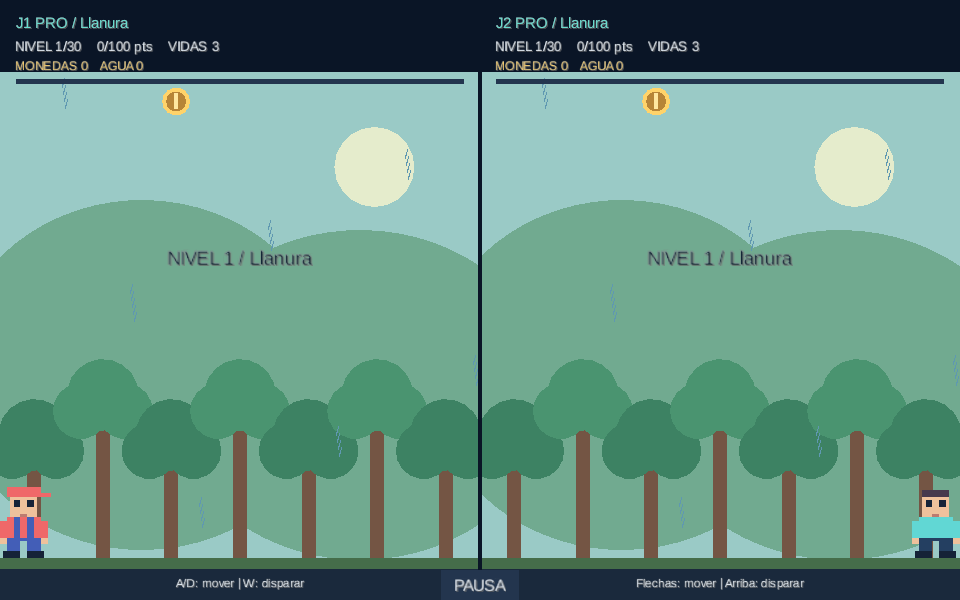
\includegraphics[width=0.78\textwidth]{images/17-versus.png}
        };
    \end{tikzpicture}\\[0.2cm]
    {\small\sffamily\color{NavyDark!70}\textit{Figura: Modo Versus local; ambos jugadores enfrentan la misma lluvia con su propio personaje.}}
\end{center}

\begin{itemize}[itemsep=0.5em]
    \item \textbf{Jugador 1 (Lado Izquierdo):} Se desplaza con las teclas \textbf{\texttt{A}} y \textbf{\texttt{D}}, y dispara contra el jefe o activa su arma con la tecla \textbf{\texttt{W}}.
    \item \textbf{Jugador 2 (Lado Derecho):} Se desplaza con las \textbf{\texttt{FLECHAS IZQ / DER}}, y dispara con la tecla \textbf{\texttt{FLECHA ARRIBA}}.
    \item \textbf{Condición de Victoria:} Ambos jugadores comparten la misma semilla de aleatoriedad de lluvia. Gana el jugador que sobreviva cuando su rival agote sus vidas, o quien logre destruir primero a su respectivo jefe espacial.
\end{itemize}

\subsection*{El Desafío Secreto del Alien (Easter Egg)}

Para los recolectores más curiosos, el juego esconde un acceso confidencial directo:

\begin{consejo}{Cómo Activar el Desafío Oculto del Alien}
    En la pantalla del \textbf{Menú Principal}, sitúe el cursor en la esquina superior izquierda extrema (coordenadas del mundo lógico; cambian en pantalla al redimensionar \texttt{X: 3, Y: 570}) y haga clic sobre el micro-botón invisible. \\
    Se iniciará inmediatamente una batalla espacial directa contra el \textbf{Jefe OVNI} en dificultad \textbf{PRO}, equipándote con \textbf{40 cargas de agua iniciales}. Este desafío no altera dinero, ranking ni niveles guardados de campaña. Si logras derrotar a la nave bajo estas condiciones, desbloquearás la skin legendaria secreta: el \textbf{Alien}.
\end{consejo}

\newpage

% ==============================================================================
% SECCION 5: INTERFAZ DE USUARIO (HUD Y MENUS)
% ==============================================================================
\section{Interfaz de Usuario (HUD y Menús)}
\label{sec:interfaz}

La interfaz gráfica de usuario (GUI) ha sido diseñada con un estilo arcade moderno de alto contraste, ofreciendo información vital al instante para que el jugador nunca pierda de vista la acción.

\subsection*{Análisis del Head-Up Display (HUD) en Partida}

\begin{center}
    \begin{tikzpicture}
        \node[inner sep=0pt, rounded corners=3mm, draw=CyanGlow, line width=1.5pt] (pantalla) {
            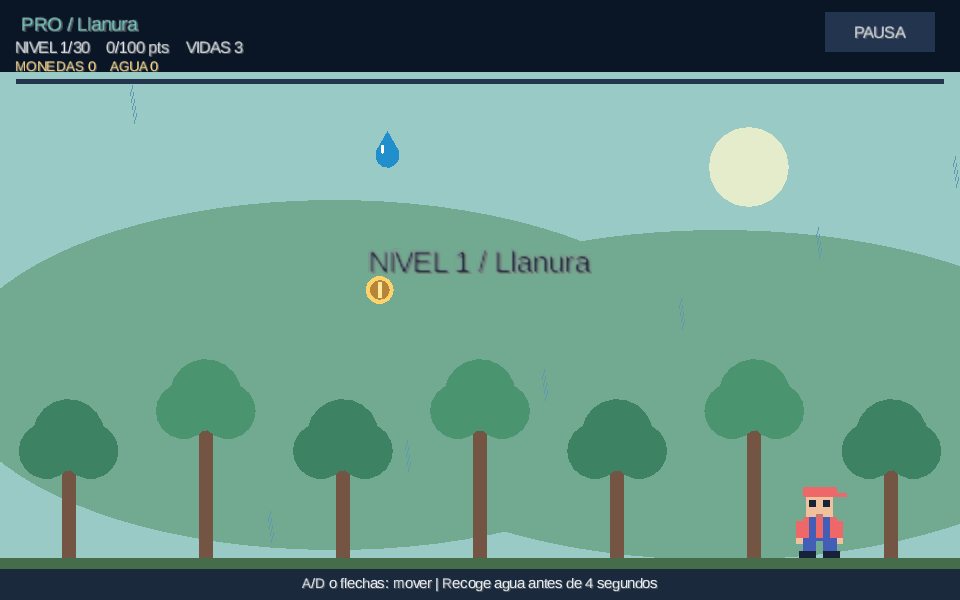
\includegraphics[width=0.88\textwidth]{images/02-partida.png}
        };
        \node[fill=NavyDark, text=CyanBright, font=\bfseries\sffamily\scriptsize, rounded corners=1mm, draw=CyanGlow] 
            at ($(pantalla.north west)+(2.2cm,-0.6cm)$) {[1] Puntuación Actual};
            
        \node[fill=NavyDark, text=GoldDrop, font=\bfseries\sffamily\scriptsize, rounded corners=1mm, draw=GoldDrop] 
            at ($(pantalla.north)+(0cm,-0.6cm)$) {[2] Nivel y Bioma / Agua};
            
        \node[fill=NavyDark, text=RedAlert!40!white, font=\bfseries\sffamily\scriptsize, rounded corners=1mm, draw=RedAlert] 
            at ($(pantalla.north east)+(-2.2cm,-0.6cm)$) {[3] Vidas y Monedas};
            
        \node[fill=NavyDark, text=white, font=\bfseries\sffamily\scriptsize, rounded corners=1mm, draw=white!60] 
            at ($(pantalla.north east)+(-1.2cm,-1.5cm)$) {[4] Botón de Pausa};
    \end{tikzpicture}\\[0.2cm]
    {\small\sffamily\color{NavyDark!70}\textit{Figura: Elementos informativos desplegados en tiempo real durante la partida.}}
\end{center}

\begin{enumerate}[label=\textbf{[\arabic*]}, itemsep=0.8em]
    \item \textbf{Marcador de Puntos (Extremo Superior Izquierdo):}\\
    Muestra la puntuación acumulada durante la sesión. El agua normal aporta 10 puntos. Agua doble, oasis, multiplicadores y perjuicios cambian la relación entre gotas y puntuación. Si este valor llega a múltiplos de $100$ ($100, 200, 300\dots$), el sistema incrementa automáticamente tu nivel de campaña.
    
    \item \textbf{Panel Central de Nivel, Bioma y Reserva de Agua:}\\
    Indica el nivel en el que te encuentras (del $1$ al $30$) y el bioma activo (Llanura, Hielo o Desierto). A su vez, muestra las \textbf{cargas de agua} disponibles en tu recolector, necesarias para disparar al jefe. Recoger agua restaura la hidratación; disparar no modifica la sed.
    
    \item \textbf{Contador de Vidas y Monedas (Extremo Superior Derecho):}\\
    Representa las vidas que le quedan al personaje antes de caer derrotado. Junto a las vidas, se contabilizan las monedas doradas obtenidas en la tormenta, las cuales se transfieren a tu billetera permanente para gastar en la tienda.
    
    \item \textbf{Acceso Rápido a Pausa:}\\
    Un botón interactivo que detiene la acción si necesitas un respiro o deseas salir guardando las monedas. Abandonar no registra el puntaje en el ranking.
\end{enumerate}

\subsection*{Pantallas de Navegación y Menús Secundarios}

\begin{figure}[h!]
    \centering
    \begin{subfigure}[b]{0.48\textwidth}
        \centering
        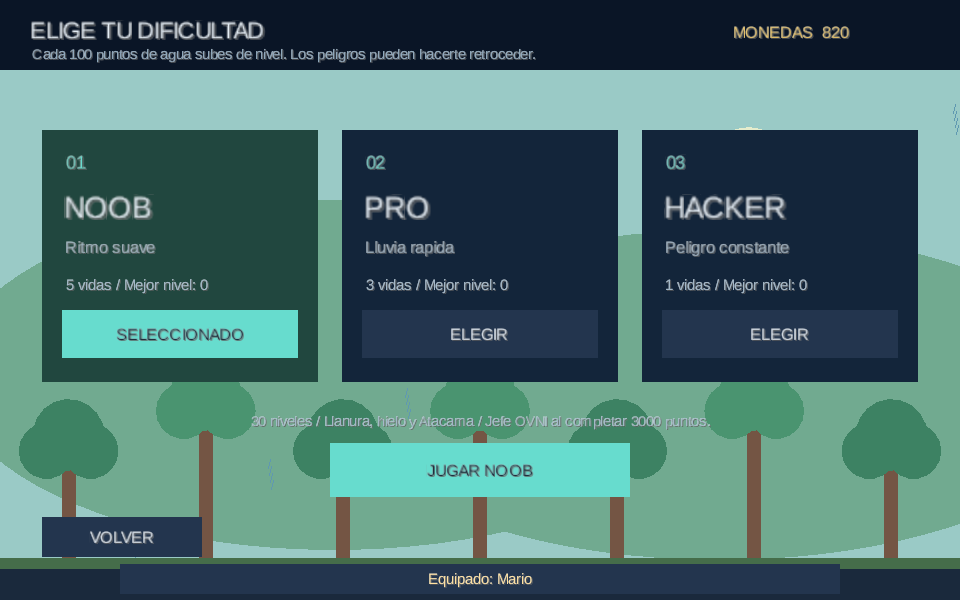
\includegraphics[width=\textwidth]{images/07-dificultad.png}
        \caption{Selector de Dificultad y récord histórico}
    \end{subfigure}
    \hfill
    \begin{subfigure}[b]{0.48\textwidth}
        \centering
        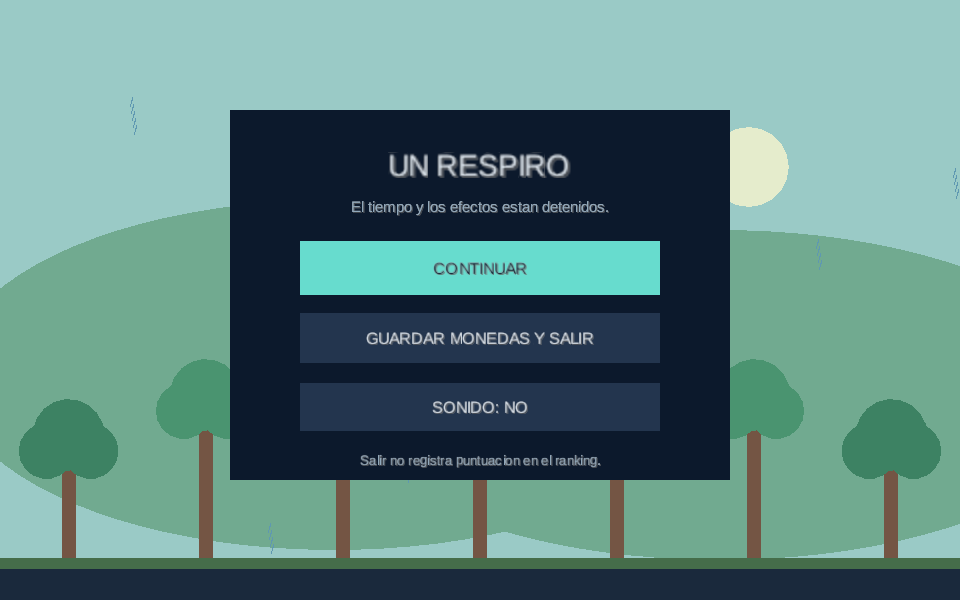
\includegraphics[width=\textwidth]{images/03-pausa.png}
        \caption{Menú de Pausa en medio de la partida}
    \end{subfigure}
    \par\vspace{0.3cm}
    \begin{subfigure}[b]{0.48\textwidth}
        \centering
        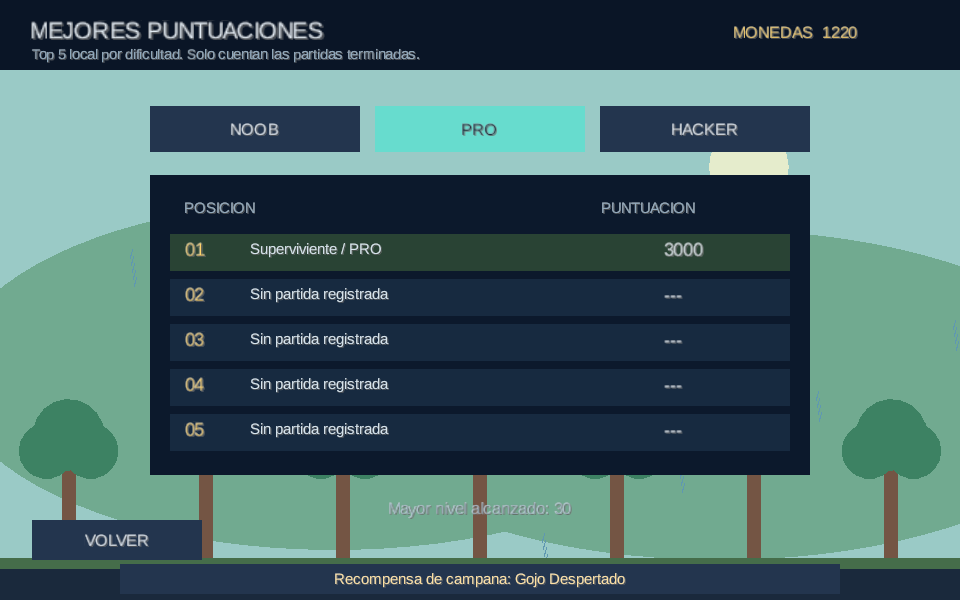
\includegraphics[width=\textwidth]{images/10-puntuaciones.png}
        \caption{Tabla de Mejores Récords locales (Top 5)}
    \end{subfigure}
    \hfill
    \begin{subfigure}[b]{0.48\textwidth}
        \centering
        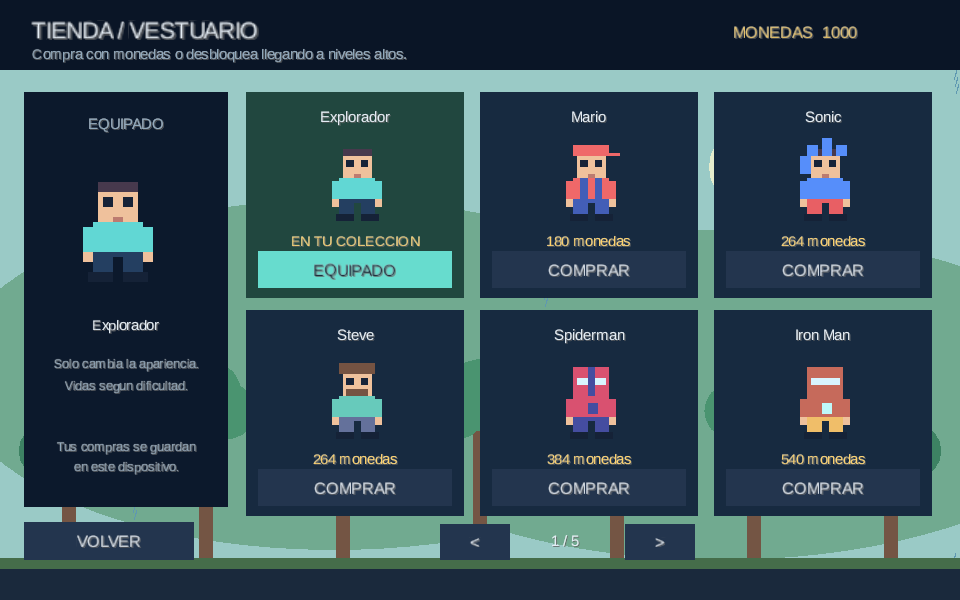
\includegraphics[width=\textwidth]{images/05-tienda.png}
        \caption{Tienda de Aspectos y Personalización}
    \end{subfigure}
    \caption{Conjunto de pantallas de configuración, progreso y personalización del juego.}
\end{figure}

\newpage

% ==============================================================================
% SECCION 6: CATALOGO DE ELEMENTOS Y PRECIPITACIONES
% ==============================================================================
\section{Catálogo de Elementos y Precipitaciones (Guía de Campo)}
\label{sec:elementos}

Al igual que en las expediciones de campo, conocer las sustancias que caen de la atmósfera es la diferencia entre la victoria y la derrota. A continuación se detalla cada elemento disponible en el juego:

\subsection*{Suministros Beneficiosos y Recursos Vitales}

\begin{tarjetaitem}{Gota de Agua Pura}{Suministro Básico Vital}
    \begin{tabularx}{\textwidth}{lX}
        \textbf{Efecto Inmediato:} & Suma \textbf{+10 puntos}, otorga \textbf{+1 carga de agua} y cura la deshidratación al instante. \\
        \textbf{Importancia:} & Es el núcleo de la jugabilidad. Sin ella no puedes avanzar de nivel ni disparar contra el OVNI.
    \end{tabularx}
\end{tarjetaitem}

\vspace{0.3cm}

\begin{tarjetaitem}{Agua Doble}{Concentrado Hídrico}
    \begin{tabularx}{\textwidth}{lX}
        \textbf{Efecto Inmediato:} & Otorga \textbf{+20 puntos} y recarga \textbf{+2 cargas de agua} en el recolector. \\
        \textbf{Importancia:} & Acelera el progreso hacia el siguiente nivel y abastece rápidamente el cañón de agua.
    \end{tabularx}
\end{tarjetaitem}

\vspace{0.3cm}

\begin{tarjetaitem}{Agua de Oasis}{Manantial de Respaldo}
    \begin{tabularx}{\textwidth}{lX}
        \textbf{Efecto Inmediato:} & Otorga \textbf{+30 puntos} de bonificación y \textbf{+3 cargas completas de agua}. \\
        \textbf{Importancia:} & Muy cotizada en el Desierto de Atacama para contrarrestar el desgaste térmico.
    \end{tabularx}
\end{tarjetaitem}

\vspace{0.3cm}

\begin{tarjetaitem}{Moneda Dorada y Monedas x2}{Economía de Campaña}
    \begin{tabularx}{\textwidth}{lX}
        \textbf{Efecto Inmediato:} & Suma monedas acumulables para comprar aspectos cosméticos en la tienda del menú. \\
        \textbf{Multiplicador:} & El ítem especial \textbf{Monedas x2} duplica todas las monedas recolectadas durante \textbf{8 segundos}.
    \end{tabularx}
\end{tarjetaitem}

\vspace{0.3cm}

\begin{tarjetaitem}{Café Caliente / Fruta de Cactus}{Estimulante de Velocidad}
    \begin{tabularx}{\textwidth}{lX}
        \textbf{Efecto Temporal:} & Incrementa la agilidad del recolector en un \textbf{+50\% ($1.5\times$)} durante \textbf{7 segundos}. \\
        \textbf{Utilidad:} & Permite cruzar la pantalla velozmente para atrapar gotas distantes en niveles avanzados.
    \end{tabularx}
\end{tarjetaitem}

\vspace{0.3cm}

\begin{tarjetaitem}{Termo Caliente}{Aislamiento Criogénico}
    \begin{tabularx}{\textwidth}{lX}
        \textbf{Efecto Temporal:} & Otorga \textbf{inmunidad térmica absoluta} contra nieve y hielo durante \textbf{8 segundos}. \\
        \textbf{Utilidad:} & Indispensable en el bioma de Tundra para no quedar paralizado en medio de ventiscas.
    \end{tabularx}
\end{tarjetaitem}

\vspace{0.4cm}

\begin{center}
    \begin{tikzpicture}
        \node[inner sep=0pt, rounded corners=3mm, draw=NavyMedium, line width=1.5pt] {
            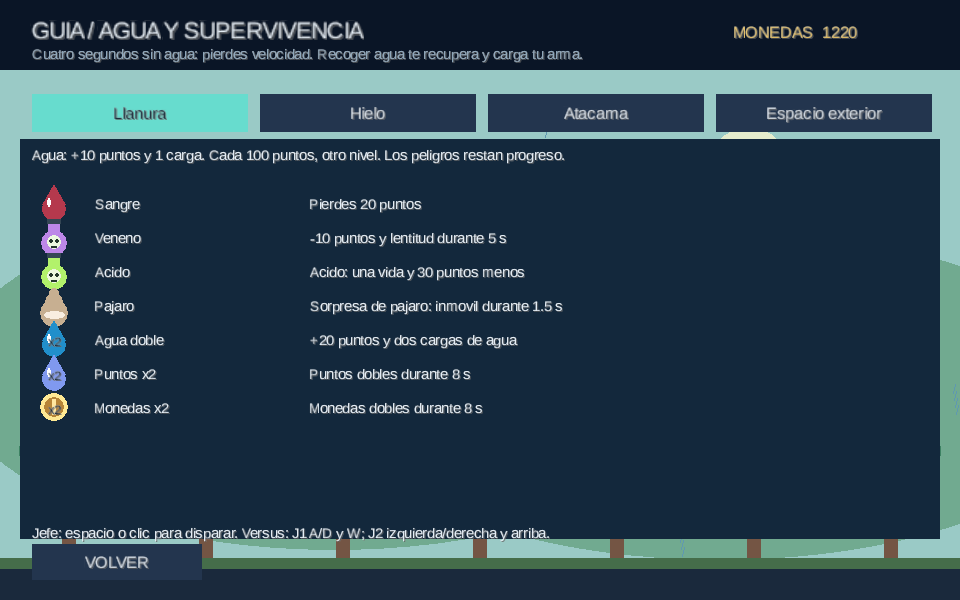
\includegraphics[width=0.85\textwidth]{images/11-guia.png}
        };
    \end{tikzpicture}\\[0.2cm]
    {\small\sffamily\color{NavyDark!70}\textit{Figura: Guía de campo interactiva accesible desde el Menú Principal con los efectos del Bioma Llanura.}}
\end{center}

\newpage

\subsection*{Peligros Atmosféricos, Toxinas y Sustancias Letales}

\begin{alerta}{¡Evita el Contacto con estos Elementos!}
    Tocar cualquiera de las siguientes sustancias acarreará penalizaciones directas a tu puntuación, inmovilidad o pérdida de vidas:
\end{alerta}

\vspace{0.3cm}

\begin{tarjetaitem}{Sangre Contaminada}{Residuo Biológico}
    \begin{tabularx}{\textwidth}{lX}
        \textbf{Penalización:} & Resta \textbf{-20 puntos} de tu marcador actual. \\
        \textbf{Impacto:} & Puede retrasar tu ascenso al siguiente nivel de campaña.
    \end{tabularx}
\end{tarjetaitem}

\vspace{0.3cm}

\begin{tarjetaitem}{Veneno}{Toxina Orgánica}
    \begin{tabularx}{\textwidth}{lX}
        \textbf{Penalización:} & Resta \textbf{-10 puntos} e intoxica al recolector, \textbf{reduciendo su velocidad al 50\%} por \textbf{5 segundos}. \\
        \textbf{Impacto:} & La lentitud acumulada dificulta esquivar peligros que caigan a continuación.
    \end{tabularx}
\end{tarjetaitem}

\vspace{0.3cm}

\begin{tarjetaitem}{Nieve y Hielo}{Fenómenos Glaciares}
    \begin{tabularx}{\textwidth}{lX}
        \textbf{Nieve:} & Resta \textbf{-20 puntos} y genera ralentización durante \textbf{4 segundos}. \\
        \textbf{Hielo:} & Resta \textbf{-30 puntos} y produce \textbf{congelamiento absoluto}, inmovilizando al jugador por \textbf{1.5 segundos}.
    \end{tabularx}
\end{tarjetaitem}

\vspace{0.3cm}

\begin{tarjetaitem}{Ácido Corrosivo}{Peligro Químico Letal}
    \begin{tabularx}{\textwidth}{lX}
        \textbf{Penalización:} & \textbf{Resta 1 VIDA DIRECTA} y descuenta \textbf{-30 puntos}. \\
        \textbf{Impacto:} & Un impacto crítico. En dificultad Hacker, recibir ácido supone la derrota inmediata.
    \end{tabularx}
\end{tarjetaitem}

\vspace{0.3cm}

\begin{tarjetaitem}{Fuego Abrasador y Cactus}{Amenazas de Combustión y Espinas}
    \begin{tabularx}{\textwidth}{lX}
        \textbf{Fuego:} & \textbf{Resta 1 VIDA DIRECTA} y descuenta \textbf{-40 puntos}. \\
        \textbf{Cactus:} & \textbf{Resta 1 VIDA DIRECTA} y descuenta \textbf{-25 puntos}. Típico de la zona de Atacama.
    \end{tabularx}
\end{tarjetaitem}

\vspace{0.3cm}

\begin{tarjetaitem}{Pájaro, Tinta y Bolsa Rota}{Interferencias Extra}
    \begin{tabularx}{\textwidth}{lX}
        \textbf{Pájaro:} & Aturde al personaje, dejándolo \textbf{inmóvil durante 1.5 segundos}. \\
        \textbf{Tinta:} & Mancha corrosiva que provoca una \textbf{pérdida masiva de 50 puntos}. \\
        \textbf{Bolsa Rota:} & Descuenta \textbf{5 monedas} e impide recoger monedas durante \textbf{4 segundos}.
    \end{tabularx}
\end{tarjetaitem}

\vspace{0.4cm}

\begin{figure}[h!]
    \centering
    \begin{subfigure}[b]{0.48\textwidth}
        \centering
        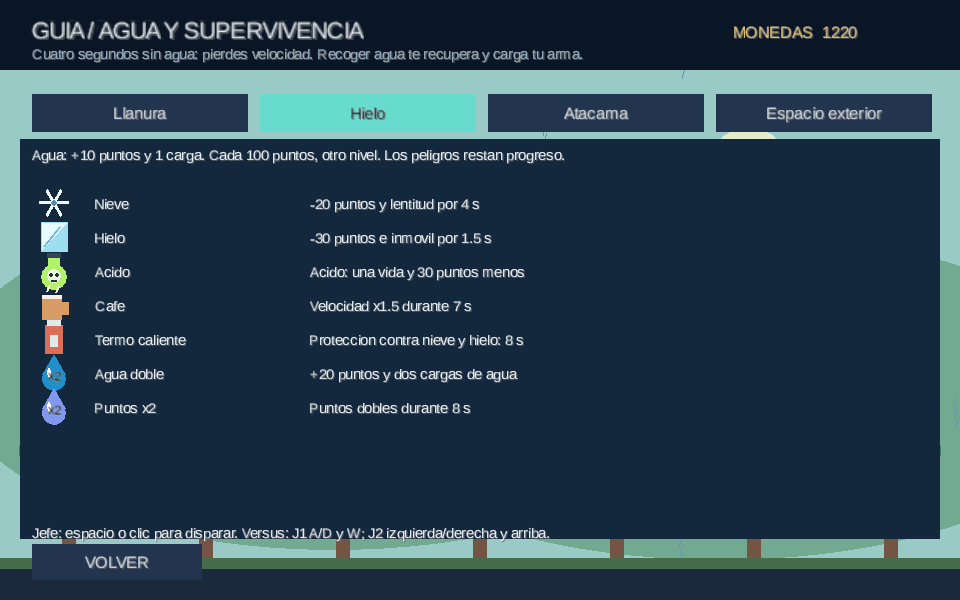
\includegraphics[width=\textwidth]{images/19-guia-hielo.png}
        \caption{Catálogo de peligros del Bioma Hielo}
    \end{subfigure}
    \hfill
    \begin{subfigure}[b]{0.48\textwidth}
        \centering
        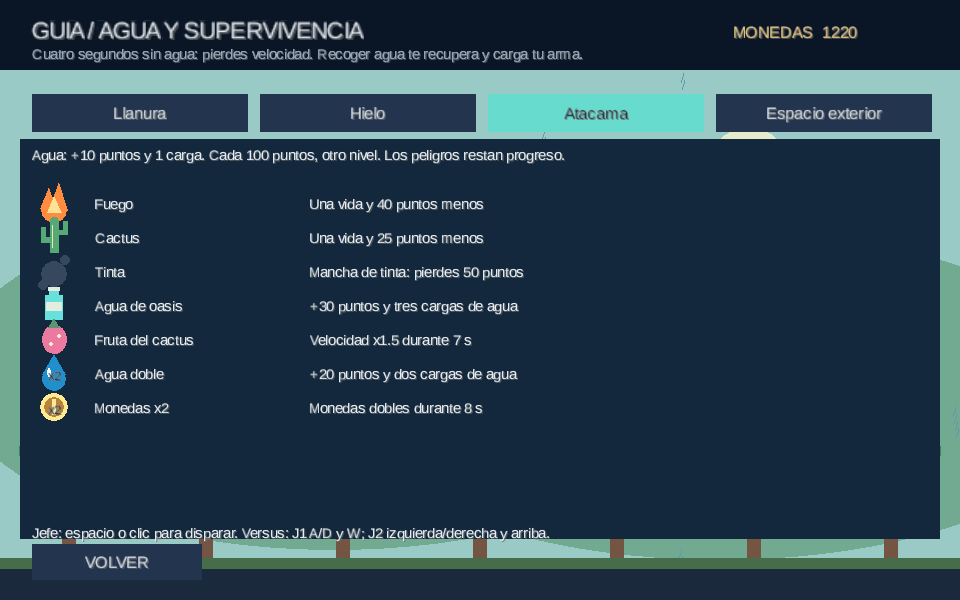
\includegraphics[width=\textwidth]{images/20-guia-desierto.png}
        \caption{Catálogo de peligros del Desierto de Atacama}
    \end{subfigure}
    \caption{Guías de peligros específicas por zona climática dentro del juego.}
\end{figure}

\newpage

% ==============================================================================
% SECCION 7: PROGRESION DE CAMPANA, BIOMAS Y JEFE FINAL
% ==============================================================================
\section{Progresión de Campaña: Biomas y Batalla Final}
\label{sec:campana}

La campaña de \textbf{GameLluvia} está estructurada como un viaje ascendente a lo largo de \textbf{30 niveles progresivos}, concluyendo en una fase de batalla final posterior al nivel 30.

\subsection*{Los Tres Biomas Terrestres}

A medida que acumulas puntos, el entorno visual y las físicas de lluvia evolucionan drásticamente:

\begin{center}
    \begin{minipage}{0.31\textwidth}
        \centering
        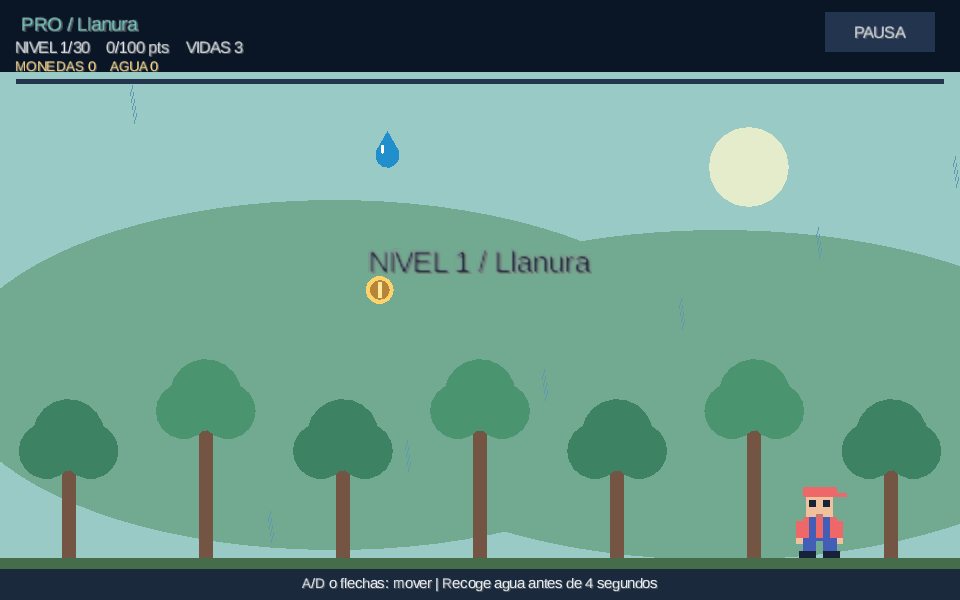
\includegraphics[width=\textwidth]{images/02-partida.png}\\[0.15cm]
        {\small\sffamily\textbf{Bioma 1: Llanura}\\(Niveles 1 al 10)\\\scriptsize Clima templado. Ideal para dominar la recolección de agua y esquivar veneno.}
    \end{minipage}
    \hfill
    \begin{minipage}{0.31\textwidth}
        \centering
        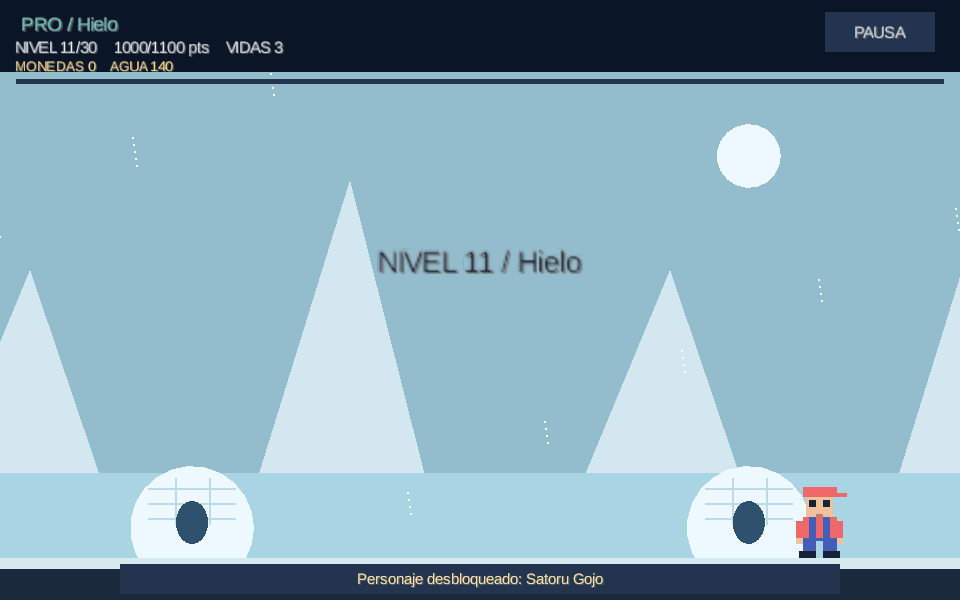
\includegraphics[width=\textwidth]{images/12-hielo.png}\\[0.15cm]
        {\small\sffamily\textbf{Bioma 2: Hielo}\\(Niveles 11 al 20)\\\scriptsize Fuertes ventiscas. El hielo y la nieve acechan; busca termos calientes.}
    \end{minipage}
    \hfill
    \begin{minipage}{0.31\textwidth}
        \centering
        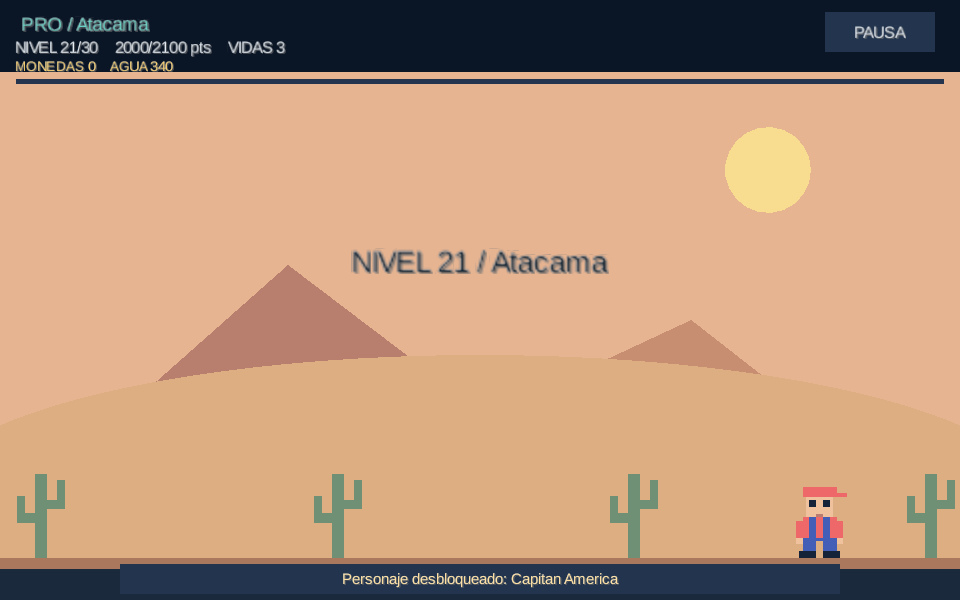
\includegraphics[width=\textwidth]{images/13-atacama.png}\\[0.15cm]
        {\small\sffamily\textbf{Bioma 3: Atacama}\\(Niveles 21 al 30)\\\scriptsize Calor extremo. Lluvia de fuego y cactus punzantes; aprovecha el oasis.}
    \end{minipage}
\end{center}

\subsection*{Rondas de Bonificación Dorada (Bonus de Monedas)}
En los niveles \textbf{5, 10, 15, 20, 25 y 30}, la atmósfera entra en una calma especial: la lluvia de contaminantes cesa durante \textbf{8 segundos completos} y caen cascadas de monedas doradas. ¡Es tu oportunidad dorada para acumular fortuna y comprar nuevas skins sin preocuparte por el daño!

\subsection*{La Confrontación Espacial: El Jefe OVNI (Fase Final)}

Al superar los \textbf{3.000 puntos} en el nivel 30, el recolector es elevado por el rayo del OVNI durante tres segundos antes del combate para enfrentarse a la nave alienígena:

\begin{center}
    \begin{tikzpicture}
        \node[inner sep=0pt, rounded corners=3mm, draw=CyanBright, line width=1.8pt] {
            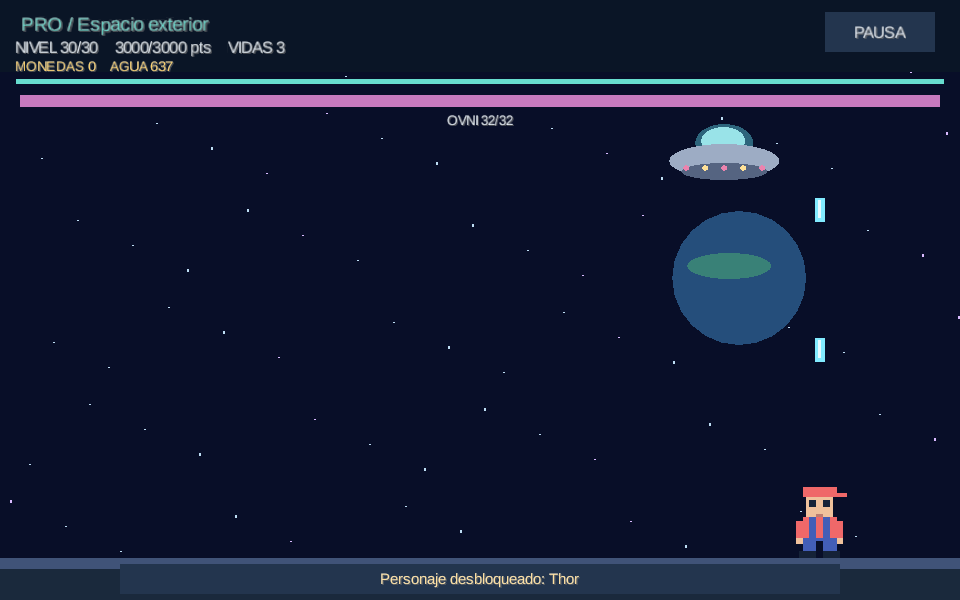
\includegraphics[width=0.8\textwidth]{images/15-jefe.png}
        };
    \end{tikzpicture}\\[0.2cm]
    {\small\sffamily\color{NavyDark!70}\textit{Figura: El Jefe OVNI disparando proyectiles en órbita mientras el jugador contraataca con agua.}}
\end{center}

\begin{itemize}[itemsep=0.6em]
    \item \textbf{Mecánica de Disparo:} El OVNI posee una barra de blindaje superior. Presiona la \textbf{Barra Espaciadora} o haz \textbf{clic izquierdo} para lanzar chorros de agua hacia arriba. Cada impacto certero reduce la salud del OVNI.
    \item \textbf{Fase de Furia (Salud al 50\%):} Al reducir la vida del jefe a la mitad, la nave entra en estado de cólera: el HUD muestra FURIA, la frecuencia de ataques y oscilación aumenta un 40\%, y los peligros caen más rápido. No se implementó un cambio de color.
    \item \textbf{Gestión del Agua en Órbita:} No olvides que cada disparo gasta 1 unidad de agua. Si vacías tu reserva, deberás maniobrar entre los disparos alienígenas para recolectar las gotas orbitales y recargar munición.
    \item \textbf{Victoria Definitiva:} Tras vaciar la salud del OVNI, se muestra la pantalla de victoria triunfal junto a una recompensa cosmética y una bolsa de 250, 400 o 550 monedas según dificultad.
\end{itemize}

\newpage

% ==============================================================================
% SECCION 8: TIENDA DE ASPECTOS Y PERSONALIZACION
% ==============================================================================
\section{Tienda de Aspectos, Personalización y Desbloqueos}
\label{sec:tienda}

El juego cuenta con un armario de \textbf{29 aspectos cosméticos (skins)} inspirados en icónicos personajes de la cultura pop, videojuegos y anime. Todos los aspectos respetan estrictamente la misma física y área de colisión para mantener la equidad competitiva.

\begin{center}
    \begin{tikzpicture}
        \node[inner sep=0pt, rounded corners=3mm, draw=GoldDrop, line width=1.5pt] {
            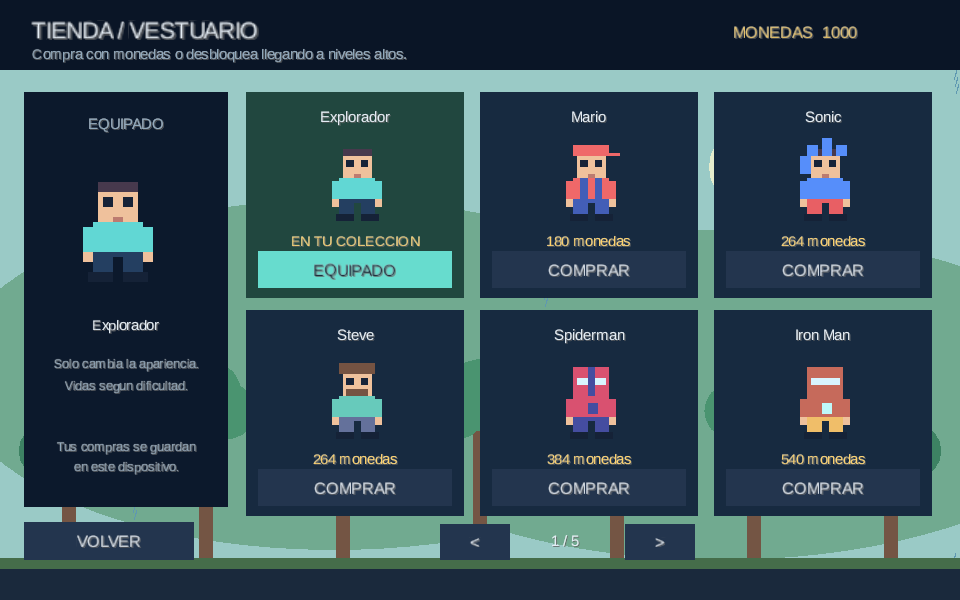
\includegraphics[width=0.78\textwidth]{images/05-tienda.png}
        };
    \end{tikzpicture}\\[0.2cm]
    {\small\sffamily\color{NavyDark!70}\textit{Figura: Catálogo interactivo de la tienda donde podrás probar y equipar tus personajes adquiridos.}}
\end{center}

\subsection*{Vías de Obtención de Personajes}

\begin{enumerate}[label=\textbf{\Alph*.}, itemsep=0.8em]
    \item \textbf{Aspectos Adquiribles con Monedas (Bolsillo de Campaña):}\\
    Se compran directamente con las monedas recolectadas en tus partidas:
    \begin{itemize}[itemsep=0.3em]
        \item \textbf{Mario} ($180$ monedas) \textcolor{NavyLight!60}{|} \textbf{Sonic} ($264$ monedas) \textcolor{NavyLight!60}{|} \textbf{Steve} ($264$ monedas)
        \item \textbf{Spiderman} ($384$ monedas) \textcolor{NavyLight!60}{|} \textbf{Iron Man} ($540$ monedas) \textcolor{NavyLight!60}{|} \textbf{Luigi} ($650$ monedas)
        \item \textbf{Alex} ($650$ monedas) \textcolor{NavyLight!60}{|} \textbf{Shadow} ($800$ monedas) \textcolor{NavyLight!60}{|} \textbf{Sasuke} ($850$ monedas)
        \item \textbf{Yuji Itadori} ($850$ monedas) \textcolor{NavyLight!60}{|} \textbf{Zoro} ($900$ monedas) \textcolor{NavyLight!60}{|} \textbf{Gohan} ($1.000$ monedas)
        \item \textbf{Among Us} ($1.100$ monedas) \textcolor{NavyLight!60}{|} \textbf{Arthur Morgan} ($1.200$ monedas) \textcolor{NavyLight!60}{|} \textbf{Pikachu} ($1.400$ monedas)
    \end{itemize}

    \item \textbf{Aspectos por Récord de Niveles (Progreso de Habilidad):}\\
    Se desbloquean automáticamente al alcanzar hitos de nivel en cada dificultad:
    \begin{itemize}[itemsep=0.3em]
        \item \textit{En NOOB:} Naruto (Nivel 10) $\cdot$ Monkey D. Luffy (Nivel 20) $\cdot$ Goku (Nivel 30).
        \item \textit{En PRO:} Satoru Gojo (Nivel 10) $\cdot$ Capitán América (Nivel 20) $\cdot$ Thor (Nivel 30).
        \item \textit{En HACKER:} Doom Slayer (Nivel 10) $\cdot$ Megumi Fushiguro (Nivel 20) $\cdot$ Vegeta (Nivel 30).
    \end{itemize}

    \item \textbf{Aspectos Legendarios por Victoria Final (OVNI Derrotado):}
    \begin{itemize}[itemsep=0.3em]
        \item Vencer al OVNI en Noob: \textbf{Goku Ultra Instinto}.
        \item Vencer al OVNI en Pro: \textbf{Gojo Despertado}.
        \item Vencer al OVNI en Hacker: \textbf{Super Sonic}.
    \end{itemize}

    \item \textbf{Aspecto Secreto Oculto:}
    \begin{itemize}
        \item \textbf{Alien:} Exclusivo tras vencer el Desafío Oculto del menú principal.
    \end{itemize}
\end{enumerate}

\newpage

% ==============================================================================
% SECCION 9: PREGUNTAS FRECUENTES Y SOLUCION DE PROBLEMAS (FAQ)
% ==============================================================================
\section{Preguntas Frecuentes y Solución de Problemas (FAQ)}
\label{sec:faq}

\begin{tarjetaitem}{¿Por qué mi personaje camina extremadamente lento de repente?}{Mecánica de Sed}
    Esto se debe al sistema de \textbf{deshidratación}. Si pasas más de 4 segundos sin recoger una gota de agua limpia, el personaje sufre fatiga y pierde hasta el 60\% de su velocidad. \\
    \textbf{Solución:} Recoge inmediatamente una gota de agua celeste (o agua doble/oasis) para restaurar al instante tu velocidad al 100\%.
\end{tarjetaitem}

\vspace{0.4cm}

\begin{tarjetaitem}{Presiono la Barra Espaciadora pero el recolector no dispara. ¿Qué ocurre?}{Munición de Agua}
    El cañón de agua a presión solo se activa en fases de combate (durante la batalla contra el Jefe OVNI en el nivel 31 tanto en campaña como en versus o desafío oculto), y \textbf{requiere tener cargas de agua en el tanque}. \\
    \textbf{Solución:} Si tu reserva de agua está en 0, esquiva los ataques alienígenas y atrapa las gotas que flotan en el espacio para recargar munición.
\end{tarjetaitem}

\vspace{0.4cm}

\begin{tarjetaitem}{¿Se pierden mis monedas y skins desbloqueadas al cerrar el juego?}{Persistencia Automática}
    \textbf{No}. Las compras y aspectos se guardan al registrarse. Las monedas de campaña se depositan al terminar o salir guardando; el ranking se actualiza al ganar o perder con puntaje positivo. El guardado se realiza mediante el componente \texttt{Preferences} de LibGDX en el disco local de tu máquina.
\end{tarjetaitem}

\vspace{0.4cm}

\begin{tarjetaitem}{La ventana del juego se ve con bandas negras laterales al maximizar.}{Ajuste de Relación de Aspecto}
    Es el comportamiento previsto por el diseño mediante \textbf{FitViewport}. Para garantizar que el área de visión y el tiempo de caída de las gotas sean exactamente iguales en monitores cuadrados, panorámicos o ultrawide, el motor preserva la relación $16:10$ sin distorsionar ni estirar los gráficos.
\end{tarjetaitem}

\vspace{0.4cm}

\begin{tarjetaitem}{El juego no inicia o la consola reporta error de Java.}{Compatibilidad JRE}
    Asegúrese de contar con Java instalado en su sistema. Abra un terminal y verifique ejecutando \texttt{java -version}. El entorno probado utiliza JDK 17. El código se compila con compatibilidad Java 11; Java 8 no puede ejecutar estas clases.
\end{tarjetaitem}

\vspace{0.8cm}

\begin{center}
    \begin{tcolorbox}[
        enhanced,
        colback=NavyDark,
        colframe=CyanBright,
        arc=3mm,
        width=0.9\textwidth,
        boxrule=1.2pt,
        halign=center
    ]
        {\sffamily\bfseries\color{white} ¡Felicitaciones! Ya conoces todas las herramientas para ser el mejor Guardián.}\\[0.15cm]
        {\sffamily\color{CyanBright} ¡Protege los recursos de la Tierra, conquista los 3 biomas y expulsa al invasor espacial!}
    \end{tcolorbox}
\end{center}

\end{document}

